\section{Derivation of Actuator Model}

\begin{figure}[t]
\centering
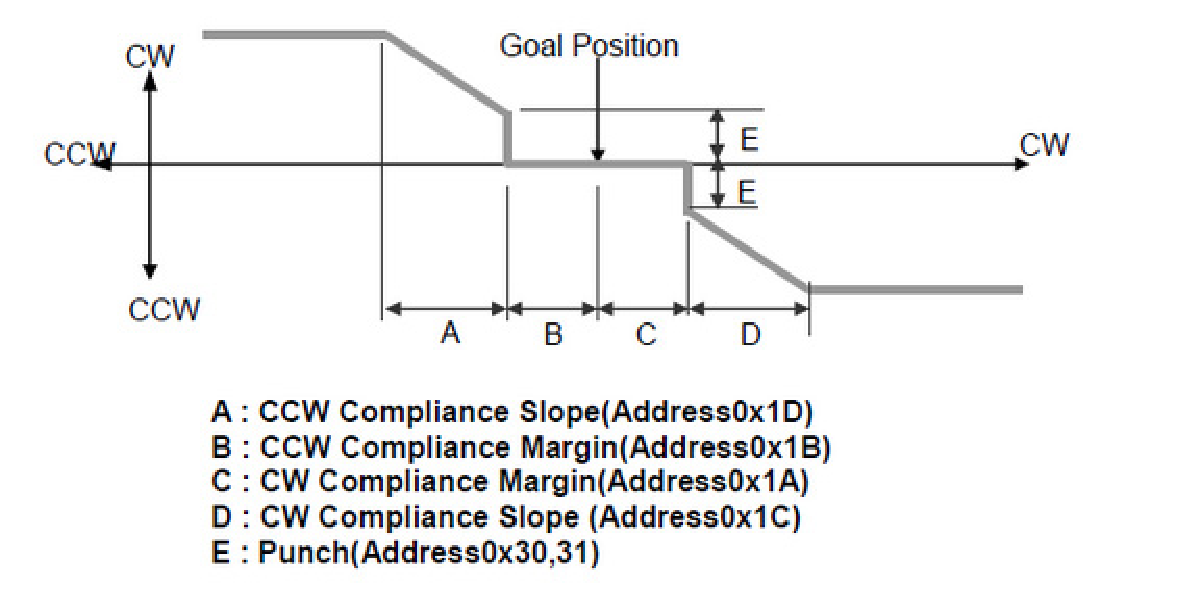
\includegraphics[width=0.45\textwidth]{figures/ax18gain.eps}
\caption{The mapping between $q-\bar{q}$ and $U$ for an AX-18 actuator \cite{AX18:2015}. The x-axis is $q-\bar{q}$ while the y-axis is $U$.}
\label{fig:actuatorMap}
\end{figure}

In this Appendix, we derive the actuator model (eq.(\ref{eqn:torqueErrorRelationSimple})) from the specifications of the Dynamixel AX-18 servo, which use the following mapping (Figure \ref{fig:actuatorMap}) between the joint angle difference $q-\bar{q}$ and the power level $U$. The intervals A and D determine the slope of the actuator response for counter-clockwise and clockwise motions respectively. Smaller values mean steeper response slopes, in which case the actuator follows the desired angle more closely. However, too small a value can lead to overshooting problems. B and C are the compliance margins. If the error of angle is within a small margin specified by B and C, the servo does not output any torque. E, the punch, is the minimum power level before the servo shuts down. In practice, we set A and D to be the same so that the servo will behave the same no matter it rotates clockwise or counter-clockwise. In addition, since B, C and E are very small compared to A and D, we ignore their effects and approximate the mapping as linear within the intervals $q-\bar{q}\in A\bigcup B\bigcup C\bigcup D$ with the slope $k_e$:
\begin{displaymath}
  U=k_e(q-\bar{q})
\end{displaymath}

To derive the relation between the power level $U$ and the output torque $\tau$, we adopt a model for the ideal DC motor \cite{SchwarzB:2013}. It is valid to assume an ideal model because the AX-18 servos use high-quality DC motors. The derivation follows by considering the power balance in the motor at a constant voltage U:
\begin{equation}
  P_{electric} = P_{mechanic} + P_{heat}
  \label{eqn:powerBalance}
\end{equation}
where $P_{electric}$ is the electrical power, $P_{mechanic}$ is the mechanical power, and $P_{heat}$ is the power dissipated as heat. From eq.(\ref{eqn:powerBalance}), we can get the following relation:
\begin{equation}
UI=\dot{q}\tau_{motor} + RI^2
\end{equation}
where $I$ is the current and $R$ is the motor winding resistance. In an ideal DC motor, the torque is linearly proportional to the current $\tau_{motor}=k_{\tau}I$. Plugging it into the above equation, we arrive at the relation between the voltage $U$ and the total torque generated by the motor $\tau_{motor}$:
\begin{equation}
  U=k_{\tau}\dot{q}+\frac{R}{k_{\tau}}\tau_{motor}
  \label{eqn:votageTorqueRelation}
\end{equation}
where $k_{\tau}$ is the torque constant, which is determined by the hardware design of the motor. The total torque generated by the motor is not yet the output torque that drives the motor shaft due to the friction inside the motor. The total torque can be decomposed into the output torque $\tau$ and the friction torque $\tau_f$.
\begin{equation}
  \tau_{motor}=\tau+\tau_f
  \label{eqn:torqueBalance}
\end{equation}
The friction torque can be further divided into viscous friction and Coulomb friction \cite{SchwarzB:2013}:
\begin{equation}
  \tau_f = k_v\dot{q}+k_c\sgn(\dot{q})
  \label{eqn:frictionComponents}
\end{equation}
where $k_v$ and $k_c$ are friction coefficients for the viscous and Coulomb friction respectively. $\sgn(x)$ is the sign function that equals 1 if $x$ is positive, -1 if $x$ is negative and 0 otherwise.

Combining eq.(\ref{eqn:votageTorqueRelation}), (\ref{eqn:torqueBalance}) and (\ref{eqn:frictionComponents}), we get the relation between the error of the joint angle $q-\bar{q}$ and the output torque $\tau$.
\begin{align}
\nonumber  \tau & = \frac{k_{\tau}k_e}{R}(q-\bar{q})+(-k_v-\frac{k_{\tau}^2}{R})\dot{q}-k_c\sgn(\dot{q})\\
\nonumber & = -k_p(q-\bar{q}) - k_d\dot{q} - k_c\sgn(\dot{q})
\end{align}
where $k_p=-\frac{k_{\tau}k_e}{R}$ and $k_d=k_v+\frac{k_{\tau}^2}{R}$. 
